\documentclass{standalone}
\usepackage{tikz}

% == Tikz
\newcommand{\drawcirc}{\node[draw,circle,minimum size=1.5cm]}
\newcommand{\drawbox}{\node[draw,rectangle,minimum size=1.5cm]}
\newcommand{\drawcircred}{\node[thick, red, draw,circle,minimum size=1.5cm]}
\newcommand{\drawcircblue}{\node[thick, blue, draw,circle,minimum size=1.5cm]}
\newcommand{\drawboxred}{\node[thick, red, draw,rectangle,minimum size=1.5cm]}
\newcommand{\drawdummy}{\node[minimum size=0,inner sep=0]}

\begin{document}
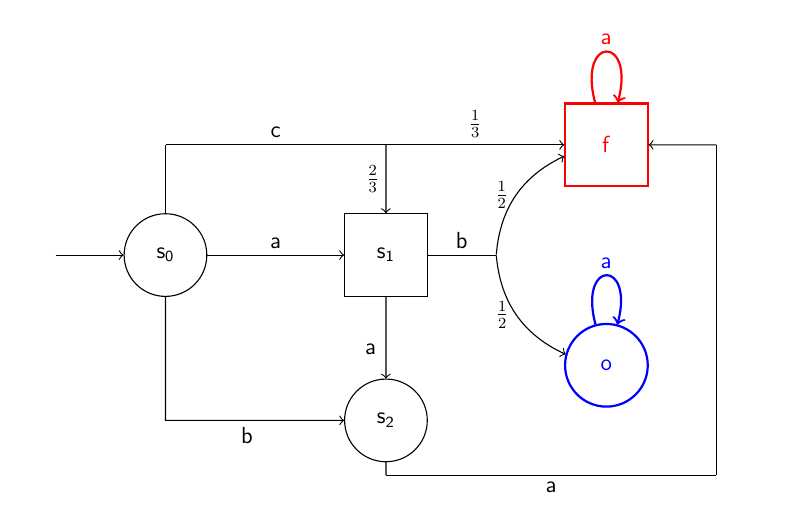
\begin{tikzpicture}[scale=0.7, every node/.style={font=\large, transform shape}]
%little BCEC with loop

\drawdummy (init) at (-2,0) {};
\drawcirc (p) at (0,0) {$\mathsf{s_0}$};
\drawdummy (pHelp) at (0,2) {};
\drawdummy (pMid) at (4,2) {};
\drawbox (q) at (4,0) {$\mathsf{s_1}$};
\drawcirc (v) at (4,-3) {$\mathsf{s_2}$};
\drawdummy (vHelp1) at (4,-4) {};
\drawdummy (vHelp2) at (10,-4) {};
\drawdummy (vHelp3) at (10,2) {};
\drawdummy (spacing) at (11,2) {};
\drawdummy (spacingleft) at (-2.5,0) {};
\drawdummy (mid) at (6,0) {};
\drawboxred (1) at (8,2) {$\mathsf{f}$};
\drawcircblue (0) at (8,-2)  {$\mathsf{o}$};

\draw[->] (init) to (p);
\draw[-] (p) to (pHelp);
\draw[-] (pHelp) to node [midway, above] {$\mathsf{c}$} (pMid);
\draw[->] (pMid) to node [midway, above] {$\frac{1}{3}$} (1);
\draw[->] (pMid) to node [midway, left] {$\frac{2}{3}$} (q);
\draw[->] (p) to node [midway,anchor=south] {$\mathsf{a}$}(q) ;
\draw[->] (p) to (0, -3) to node [text width = 0.5cm, below, midway] {$\mathsf{b}$} (v);
\draw[->] (q) to node [text width = 0.75cm, below, midway] {$\mathsf{a}$} (v);
\draw[-] (v) to (vHelp1);
\draw[-] (vHelp1) to node [below, midway] {$\mathsf{a}$} (vHelp2);
\draw[-] (vHelp2) to (vHelp3);
\draw[->] (vHelp3) to (1);
\draw[-] (q) to node [midway,anchor=south] {$\mathsf{b}$} (mid) ;
%\draw (mid) -- (0);% node [midway,anchor=north east] {0.5};
%\draw (mid) -- (1);% node [midway,anchor=south east] {0.5};
\draw[->] (mid) to [bend right] node [text width =0.25cm, left, midway] {$\frac{1}{2}$} (0);
\draw[->] (mid) to [bend left] node [text width =0.25cm, midway, left] {$\frac{1}{2}$} (1);
%\draw (mid) to [bend left,out=270,in=270] (q) ;
\draw[thick, blue,->]  (0) to[loop above]  node [midway,anchor=south] {$\mathsf{a}$} (0);
\draw[thick, red,->]  (1) to [loop above] node [midway,anchor=south] {$\mathsf{a}$} (1);
\end{tikzpicture}
\end{document}